\documentclass{article}
%% packages
\usepackage{arxiv}
\usepackage[utf8]{inputenc} % allow utf-8 input
\usepackage[T1]{fontenc}    % use 8-bit T1 fonts
\usepackage{hyperref}  
% hyperlinks
\usepackage{url}            % simple URL typesetting
\usepackage{booktabs}       % professional-quality tables
\usepackage{amsfonts}       % blackboard math symbols
\usepackage{nicefrac}       % compact symbols for 1/2, etc.
\usepackage{microtype}      % microtypography
% \usepackage{subcaption}
\usepackage{balance}  % to better equalize the last page
\usepackage{graphicx} % for EPS, load graphicx instead
% \usepackage{times}    % comment if you want LaTeX's default font
\usepackage{url}      % llt: nicely formatted URLs
\usepackage{caption}
\usepackage{soul}
\usepackage{color}
\usepackage{subfig}
\usepackage{amsmath}
\usepackage{float}
\usepackage{cleveref}
\usepackage{textcomp}
\usepackage[T1]{fontenc}
\usepackage{lineno}
\usepackage[dvipsnames]{xcolor}
\usepackage[authoryear,round]{natbib}
%% \usepackage[sorting=none,url=true,firstinits=true]{biblatex}
\usepackage{fancyhdr}

%%
%% end of the preamble, start of the body of the document source.

\begin{document}

\title{Action Affordance Affects Proximal and Distal Goal-oriented Planning}

%% \rhead{\bfseries Keshava et al. | Gaze Tool Interaction}

\author{
  Ashima Keshava\\
  University of Osnabr{\"u}ck\\
  Germany\\
  \texttt{akeshava@uos.de} \\
  %% examples of more autho
   \And
   Nina Gottschewsky\\
  University of Osnabr{\"u}ck\\
  Germany\\
  \And
   Stefan Balle\\
  University of Osnabr{\"u}ck\\
  Germany\\
  %% examples of more authors
  \And
  Farbod Nosrat Nezami\\
  University of Osnabr{\"u}ck\\
  Germany\\
  \And
   Thomas Sch{\"u}ler\\
  Halocline GmbH \& Co. KG\\
  Germany\\
  \And
   Peter K{\"o}nig\\
   University of Osnabr{\"u}ck\\
   University Medical Center,\\ Hamburg-Eppendorf\\
   Germany
}
\maketitle
\begin{abstract}
Visual attention is mainly goal-directed and allocated based on the action performed. However, it is unclear how far these results generalize to cognition in more naturalistic settings. The present study investigates active inference processes revealed by eye movements during interaction with familiar and novel tools with two levels of realism of the action affordance. In the first experiment, participants interacted with a VR controller in a low realism environment; in the second, they performed the task with an interaction setup that allowed differentiated hand and finger movements in a high realism environment. We investigated the differences in odds of fixations and their eccentricity towards the tool parts before action initiation. The results show that participants fixate more on the tool’s effector part before action initiation for the use task for unfamiliar tools. \hl{The spatial viewing bias on the tool reveals early fixations are influenced by the task and the familiarity of the tools.} Our findings show that fixations are made in a task-oriented way to plan the intended action well before action initiation. With more realistic action affordances, fixations are made towards the proximal goal of planning the grasp even though the perceived action on the tools is identical for both experimental setups. Taken together, proximal and distal goal-oriented planning is contextualized to the realism of action/interaction afforded by an environment.



\end{abstract}

\keywords{anticipatory behavior, action-oriented attention, active inference, eye-tracking, virtual reality, natural cognition}

\linenumbers
\captionsetup[figure]{font=scriptsize,labelfont=bf}
\section{Introduction}

A longstanding goal of the cognitive sciences is to understand cognition, behavior, and experience as it unfolds in the natural world \citep{Parada2020-qq}. Given the technological advancements made in the last decade, there are few methodological roadblocks to understanding natural cognition where laboratory studies can be extended to naturalistic settings and hopefully lead towards new insights \citep{Ladouce2016-li, Parada2018-vf}. More recently, a pragmatic turn has emerged in the field where there is a greater push towards incorporating the body and bodily actions to infer cognitive function \citep{Engel2013-bx}. 

Human tool use is an explicitly natural cognitive function that involves the transfer of proximal goals (e.g., placement of grasp) to distal goals for the tool \citep{Arbib2009-wa}.  Moreover, simple tools fundamentally expand the body representations to include representations of the tool in the peripersonal space \citep{Berti2000-ap, Farne2005-ns, Maravita2002-sq}. Furthermore, tool use is differentiated from other object-based actions where the tool is “acted with” \citep{Johnson2003-ee} and requires semantic knowledge of the tool as well as the necessary skill to perform actions with it \citep{Johnson-Frey2004-qk}. Hence, tool use involves complex behaviors ranging from cognitive and semantic reasoning to perceptual and motor processing.

When using tools, a wealth of information is parsed to produce the relevant action. The semantic knowledge associated with the tool helps understand how it is used, the mechanical knowledge maps the physical properties of the tool for potential usage, and finally, sensorimotor knowledge helps decipher possible movements required to use the tool \citep{Baumard2014-kv}. The amalgamation of these knowledge sources (which can be unique to a tool) necessitates planning any action associated with the tool. When this knowledge is not readily available, inferential processes must be deployed to deduce the relevant action. 

\citet{Henderson2017-tx} proposed that gaze control in natural scene can be characterized as the result of knowledge-driven predictions. These predictions for gaze control are based on the knowledge gained from past experiences. Predictive gaze control aims to sample informative and meaningful information in the environment that is relevant to the current needs of the cognitive system. Furthermore, gaze control proactively samples information in anticipation of the following action \citep{Hayhoe2004-ni, Land2001-do, Pelz2001-cn}. \citet{Belardinelli2016-kf}  showed that eye movements are goal-oriented and are modulated in anticipation of the object interaction task. There is strong evidence that task plays a vital role in how the eyes scan the scene and are differentiated between passive viewing and pantomimed interaction \citep{Belardinelli2015-in}. Similarly, \citet{Keshava2020-cp} showed that rudimentary object interactions can be predicted using eye-movement data alone. Even in the absence of an active interaction, task relevance plays an important role \citep{Castelhano2009-px, Henderson2017-it}. These studies point towards gaze control being the consequence of knowledge and task-driven predictions.

In a similar vein, \citet{Belardinelli2016-xb} investigated the role of anticipatory eye movements when interacting with familiar and unfamiliar tools in a controlled lab setting. These tools had differentiable parts: tool handle and effector. The results showed that in the case of unfamiliar tools, preparatory fixations are made on the tool-effector to extract the mechanical properties of the tool as the semantic information was not readily available. This effect was enhanced when subjects were asked to perform tool-specific movements instead of a generic action of lifting the tool by the handle. The authors, hence, concluded that eye movements are used to actively infer the appropriate usage of the tools from their mechanical properties. In the study, the tools were presented as images on a screen, and participants pantomimed lifting or using the tool. While the study revealed valuable insights into anticipatory gaze control, a question remains if these results are part of natural cognition and can be reproduced in more realistic environments.

\citet{Herbort2011-hf}  further investigated the interaction of habitual and goal-directed processes that affect grasp selection while interacting with everyday objects. They presented objects in different orientations and showed that grasp selection depended on the overarching goal of the movement sequence dependent on the object’s orientation. \citet{Belardinelli2016-kf} further showed that fixations have an anticipatory preference for the region where the index finger is placed. Consequently, the location of fixations is predictive of both proximal goals of manual planning and task-related distal goals.

When studying anticipatory behaviors corresponding to an action, there must be a distinction of symbolized or pantomimed vs. real actions. \citet{Kroliczak2007-wo} showed brain areas typically involved in real actions are not driven by pantomimed actions and that pantomimed grasps do not activate the object-related regions within the ventral stream. Similarly, \citet{Hermsdorfer2012-ca} showed a weak correlation between the hand trajectories for pantomimed and actual tool interaction. These studies indicate that the realism of sensory and tactile feedback while acting (e.g., a grasp) can be an essential factor when studying anticipatory behavioral control.

As research steadily moves towards a more ecological view of cognitive processing with bodily actions and interactions with the environment, there is a greater need to understand behavioral differences induced by varying degrees of realism of action affordances. \citet{Chalmers2008-vr} posit that defining levels of realism is necessary to achieve a one-to-one mapping of an experience in the virtual environment with the same experience in the real environment. Moreover, for research purposes such one-to-one mapping is necessary to avoid misrepresenting the real environment. In virtual reality (VR), realistic actions can be produced by different kinds of interaction methods. Using interfaces such as VR controllers, ego-centric visual feedback of a hand can be simulated. These interfaces usually consist of hand-held devices that are tracked in space and through which different actions are controlled by pressing buttons. One advantage of controller-based VR interaction is the possibility of haptic feedback. However, a disadvantage is that the actual hand posture while holding the controller does not necessarily correspond to the user’s simulated hand as they perform the action. Conversely, camera-based interaction interfaces such as LeapMotion, capture the real-time movements of the user’s hand and finger gestures, like wrap grasp or pinch grasp, to control different actions in the environment. These interfaces give the user a realistic simulation of their finer hand and finger movements, while they cannot give direct haptic feedback of the gripped object. Consequently, the chosen method of interaction in VR can afford different levels of realism and could elicit different behavioral responses.

In the present study, we investigated anticipatory gaze control pertaining to tool interactions in two different experiments. We were interested in the extent to which the action affordance and the environment modified active inference processes exhibited in gaze behavior. In experiment-I, subjects performed the experiment in a low realism environment and interacted with the tool models using a VR controller, which mimicked grasp in the virtual environment by pulling the index finger. In experiment-II, subjects were immersed in a high realism setting where they interacted with the tools using LeapMotion, which required natural hand and finger movements. Thus, the action affordance appeared closer to the real-world. Furthermore, in both experiments, participants interacted with 3D models of tools by lifting or using them in VR. For the stimuli set, we used familiar or unfamiliar tools as described in \citet{Belardinelli2016-xb}. Additionally, to differentiate between proximal and distal goal planning, we manipulated the spatial orientation of the tool handle so that they were either congruent or incongruent to the subjects’ handedness.  With this experimental design, we investigate the influence of task, tool familiarity, the spatial orientation of the tool, and, notably, the impact of the action affordance on anticipatory gaze behavior. 


\section{Methods}

\begin{figure}[!h]
    \centering
    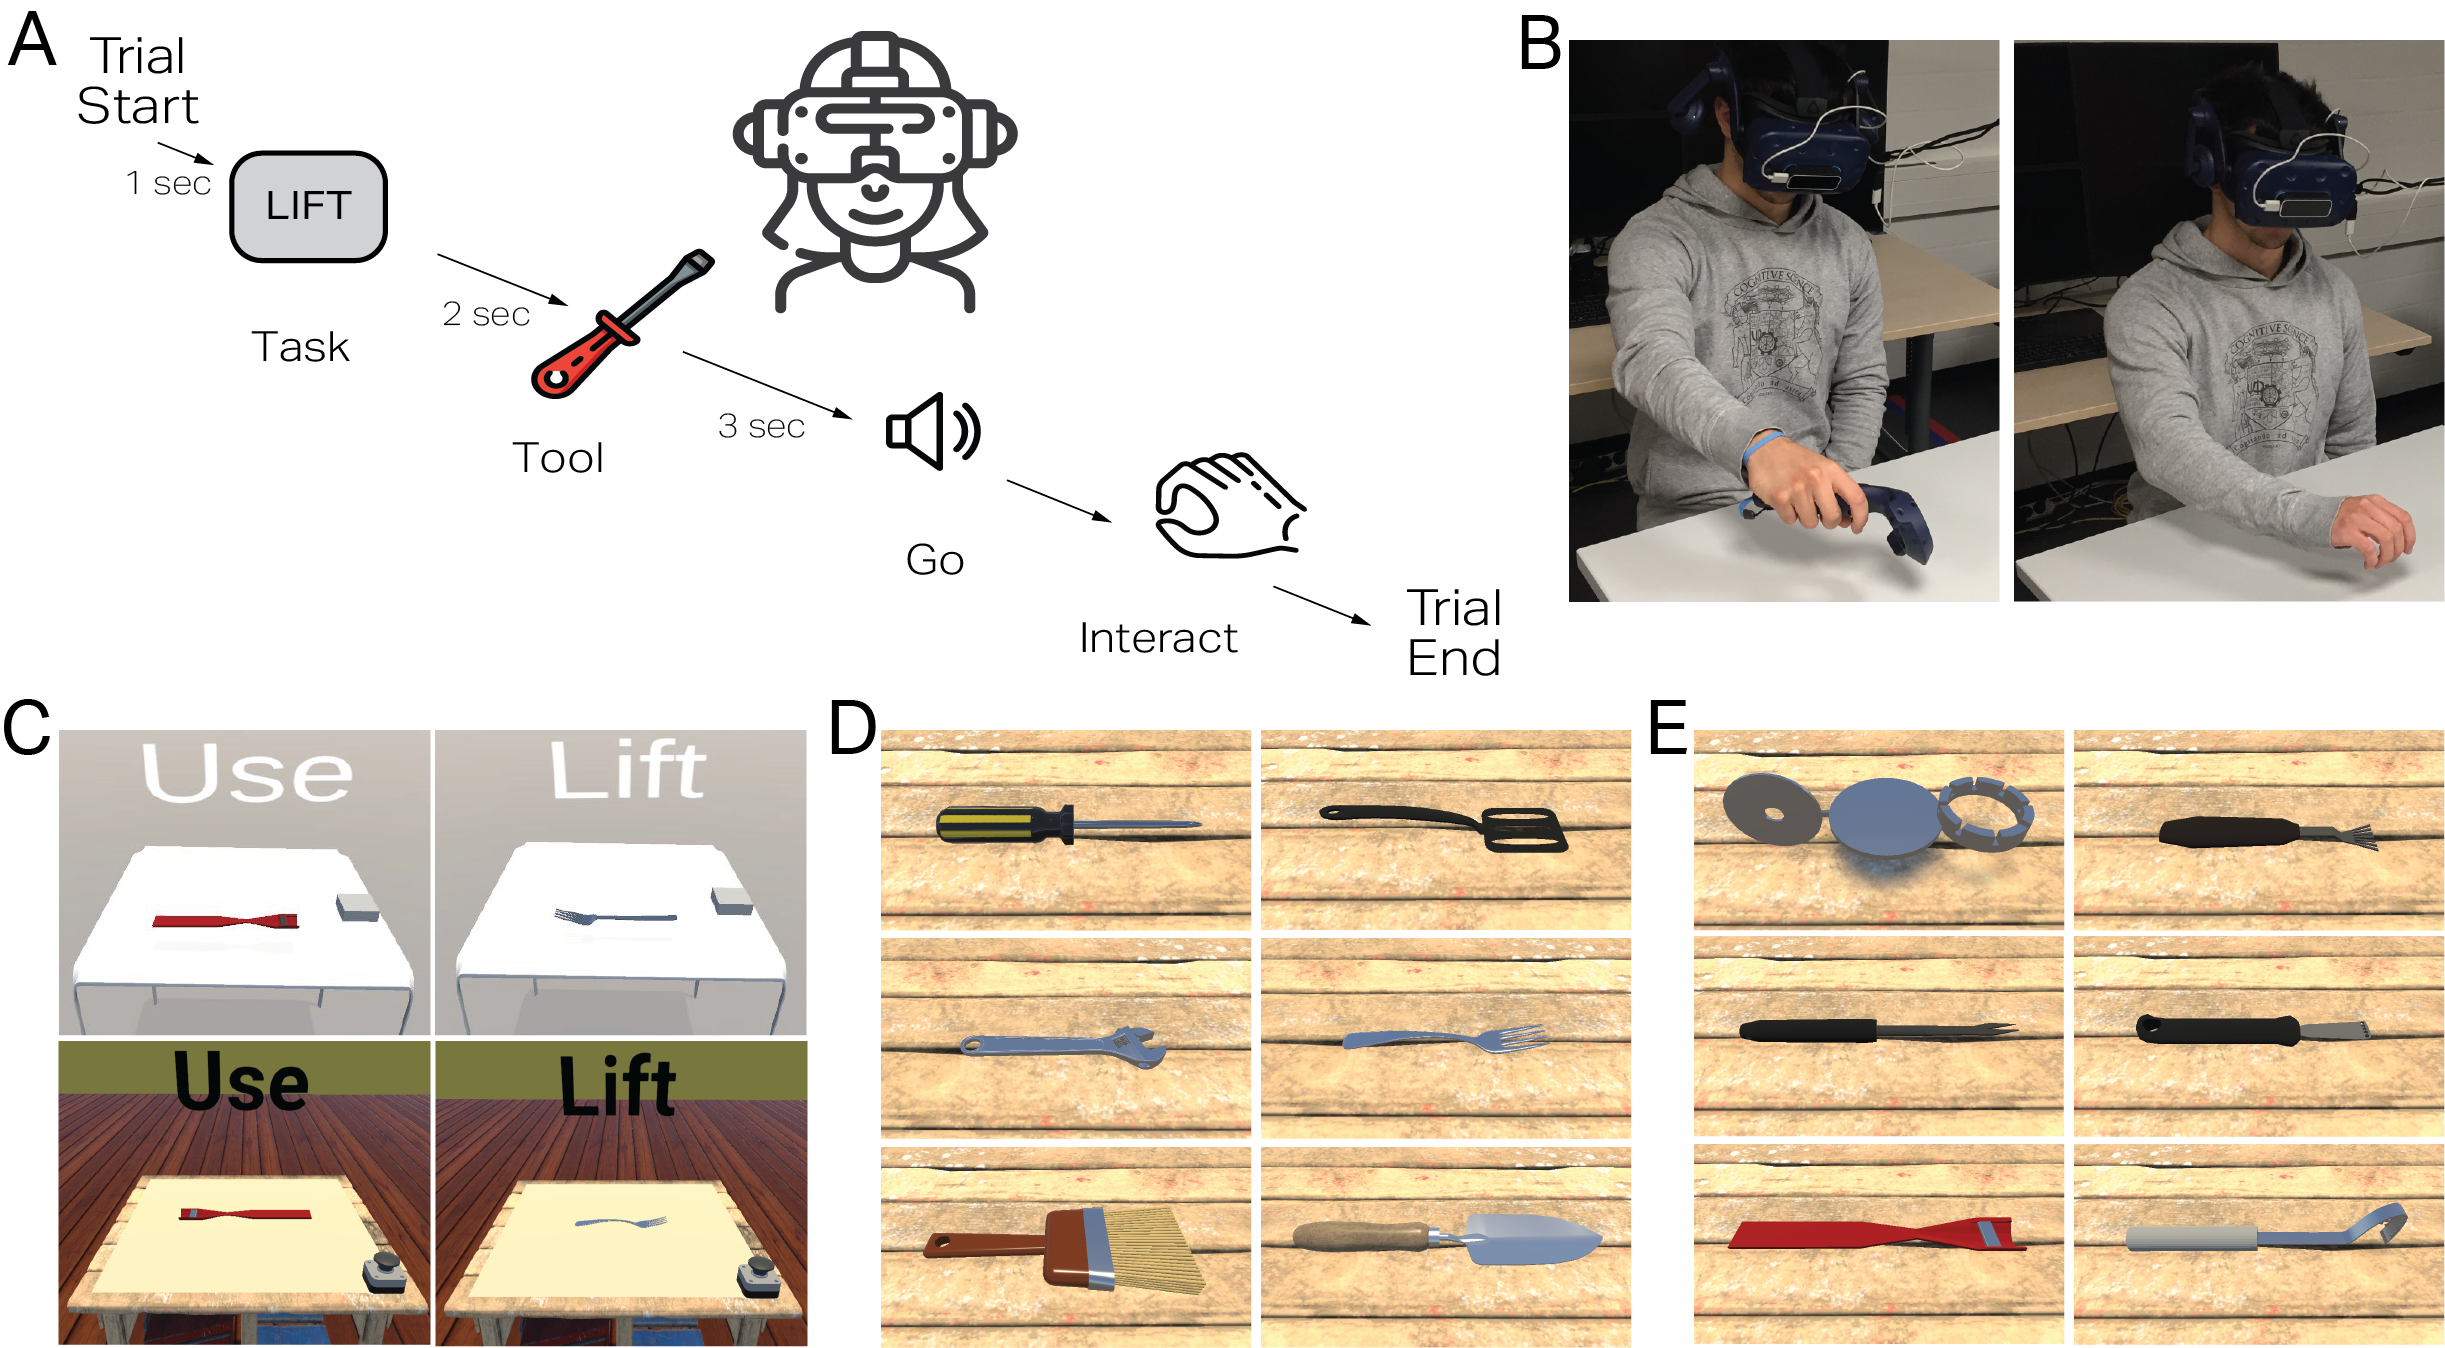
\includegraphics[width=1\linewidth]{source/figures/setup/Methods_1.png} \\
    \caption[]{Experimental Task. In two virtual environments participants interacted with tools in two ways (LIFT, USE). The tools were categorized based on familiarity (FAMILIAR, UNFAMILIAR) and presented to the participants in two orientations (HANDLE LEFT, HANDLE RIGHT). The two virtual environments differed based on the mode of interaction and perceived realism, wherein in one experiment, subjects’ hand movements were rendered virtually using the HTC-VIVE controllers. In the other experiment, the hands were rendered using LeapMotion, allowing finer hand and finger movements. \textbf{Panel A} shows the timeline of a trial. \textbf{Panel B} shows a subject in real-life performing the task in the two experiments. \textbf{Panel C} shows the differences in realism in the two experiments; TOP panels correspond to experiment with the controllers, the USE and LIFT conditions for an UNFAMILIAR and FAMILIAR tool, respectively with the tool handles presented in two different orientations. BOTTOM panels illustrate the three different conditions in a more realistic environment with LeapMotion as the interaction method. \textbf{Panel D} Familiar tools, from top-left: screwdriver, spatula, wrench, fork, paintbrush, trowel. \textbf{Panel E} Unfamiliar tools, from top-left: spoke-wrench, palette knife, daisy grubber, lemon zester, flower cutter, fish scaler.
    }
    \label{figure:task}
\end{figure}

\subsection{Experimental Task}

Subjects were seated in a virtual environment where they had to interact with the presented tool by either lifting or pretending its use.  The time course of the trials is illustrated in Figure \ref{figure:task}A. At the start of a trial, subjects saw the cued task for 2 sec after which the cue disappeared, and a tool appeared on the virtual table. Subjects were given 3 sec to view the tool, after which there was a beep (go cue) which indicated that they could start manipulating the tool based on the cued task. Subjects were seated in a virtual environment where they had to interact with the presented tool by either lifting or pretending its use. After interacting with the tool, subjects pressed a button on the table to start the next trial.  

\subsection{Participants}

For experiment-I with the HTC Vive controller’s interaction method, we recruited 18 participants ( 14 females, mean age=23.68, SD=4.05 years). For experiment-II with the interaction method of LeapMotion, we recruited 30 participants (14 female, mean age=22.7, SD=2.42 years).  All participants were recruited from the University of Osnabr{\"u}ck and the University of Applied Sciences Osnabr{\"u}ck. Participants had a normal or corrected-to-normal vision and no history of neurological or psychological impairments. All of the participants were right-handed. They either received a monetary reward of C10 or one participation credit per hour. Before each experimental session, subjects gave their informed consent in writing. They also filled out a questionnaire regarding their medical history to ascertain they did not suffer from any disorder/impairments which could affect them in the virtual environment. Once we obtained their informed consent, we briefed them on the experimental setup and task.

\subsection{Experimental Design and Procedure}

The two experiments differed based on the realism of the action affordance and the environment. Figure \ref{figure:task}B illustrates the physical setup of the participants for the two experiments. In experiment-I, subjects interacted with the tool models using the HTC Vive VR controllers. While in experiment II, subjects’ hand movements were captured by LeapMotion. 

Figure \ref{figure:task}C  illustrates two exemplar trials from the experiments. We used a 2x2x2 experimental design for both experiments, with factors task, tool familiarity, and handle orientation. Factor task had two levels: LIFT and USE. In the LIFT conditions, we instructed subjects to lift the tool to their eye level and place it back on the table. In the USE task, they had to pantomime using the tool to the best of their knowledge. Factor familiarity had two levels, FAMILIAR and UNFAMILIAR, which corresponded to tools either being everyday familiar tools or tools that are not seen in everyday contexts and are unfamiliar. The factor handle orientation corresponded to the tool handle, which was presented to the participants either on the LEFT or the RIGHT. Both experiments had 144 trials per participant, with an equal number of trials corresponding to the three factors. Subjects performed the trials over six blocks of 24 trials each. 
We measured the eye movements and hand movements simultaneously while subjects performed the experiment. We calibrated the eye-trackers at the beginning of each block and ensured that the calibration error was less than 1 degree of the visual angle. At the beginning of the experiment, subjects performed three practice trials with a hammer to familiarize themselves with the experimental setup and the interaction method. Each experiment session lasted for approximately an hour. After that, subjects filled out a questionnaire to indicate their familiarity with the 12 tools used in the experiment. They responded to the questionnaire based on a scale of 5-point Likert-like scale where 1 corresponded to “I have never used it or heard about it,” and 5 referred to “I see it every day or every week.”

\subsection{Experimental Stimuli}

The experimental setup consisted of a virtual table that mimicked the table in the real world. The table’s height, width, and length were 86cm, 80cm, and 80cm, respectively. In experiment-I, subjects were present in a bare room with grey walls and constant illumination. They sat before a light grey table, with a dark grey button on their right side to indicate the end of the trial. Similarly, in experiment-II, subjects were present in a more immersive, realistic room. They sat in front of a wooden workbench with the exact dimensions of the real-world table and a buzzer on the right to indicate the end of a trial. We displayed the task (USE or LIFT) over the desk 2m away from the participants for both experiments. 

For both experiments, we used the tool models as presented in \citet{Belardinelli2016-xb}. Six of the tools were categorized as familiar (Figure \ref{figure:task}D) and the other six as unfamiliar (Figure \ref{figure:task}E). We further created bounding box colliders that encapsulated the tools to capture the gaze position on the tool models. The mean length of the bounding box was 34.04cm (SD=5.73), mean breadth=7.60cm (SD=3.68) and mean height= 4.17cm (SD=2.13). To determine the tool effector and tool handle regions of interest, we halved the length bounding box colliders from the center of the tool and took one half as the effector and the other half as the handle. This way we refrained from making arbitrary-sized regions-of-interest for the different tool models. 

\subsection{Apparatus}
For both experiments, we used an HTC Vive head-mounted display (HMD)($110^\circ$ field of view, 90Hz, resolution 1080 x 1200 px per eye) with a built-in Tobii  eye-tracker \footnote{\href{https://enterprise.vive.com/us/product/vive-pro-eye/}{https://enterprise.vive.com/us/product/vive-pro-eye-office/}}. The HTC Vive Lighthouse tracking system provided positional and rotational tracking and was calibrated for a 4m x 4m space. For calibration of the gaze parameters, we used 5-point calibration function provided by the manufacturer. To make sure the calibration error was less than $1^\circ$, we performed a 5-point validation after each calibration. Due to the nature of the experiments, which allowed a lot of natural head movements, the eye tracker was calibrated repeatedly during the experiment after each block of 48 trials. We designed the experiment using the Unity3D game engine \footnote{\href{www.unity.com}{Unity, www.unity.com}} (v2019.2.14f1) and controlled the eye-tracking data recording using HTC VIVE Eye Tracking SDK SRanipal\footnote{\href{https://developer.vive.com/resources/vive-sense/sdk/vive-eye-tracking-sdk-sranipal/}{SRanipal, developer.vive.com/resources/vive-sense/sdk/vive-eye-tracking-sdk-sranipal/}} (v1.1.0.1)

For experiment-I, we used HTC Vive controller\footnote{\href{https://valvesoftware.github.io/steamvr_unity_plugin/articles/Quickstart.html}{SteamVR, https://valvesoftware.github.io/steamvr\_unity\_plugin/articles/Quickstart.html}} (version 2.5) to interact with the tool. The controller in the virtual environment was rendered as a gloved hand. When participants pulled the trigger button of the controller with their right index finger, their right virtual hand made a power grasp action. To interact with the tools, subjects pulled the trigger button of the controller over the virtual tools and the rendered hand grasped the tool handle. *Supplementary material video link*

Similarly, in experiment-II, we used LeapMotion\footnote{\href{https://developer.leapmotion.com/unity}{LeapMotion Unity modules, https://developer.leapmotion.com/unity}} (version 4.4.0)  to render the hand in the virtual environment. Here, subjects could see the finer hand and finger movements of their real-world movements rendered in the virtual environment. When participants made a grasping action with their hand over the virtual tool handle, the rendered hand grasped the tool handle in the virtual environment.*Supplementary material video link*

\subsection{Data pre-processing}

\subsubsection{Data Rejection}

For both experiments, we rejected trials based on two criteria. Firstly, we rejected trials where the hand position was not recorded. Secondly, we rejected trials where the gaze position and direction vectors were not recorded or recorded as invalid. For experiment-I, we rejected 29.8\% (SD=$\pm 9.6$) of trials over 18 participants. For experiment-II, we rejected a mean of 35.5\% (SD=$\pm 19.24$) of trials over 30 participants. There was a greater rejection rate in experiment-II as the LeapMotion camera lost hand-tracking more often.

\subsubsection{Gaze Data}

As a first step, using eye-in-head 3D gaze direction vector for the cyclopean eye we calculated the gaze angles in degrees for the horizontal $\theta\textsubscript{h}$ and vertical $\theta\textsubscript{v}$ directions. All of the gaze data was sorted by the timestamps of the collected gaze samples. The 3D gaze normals are represented as $(x, y, z)$ a unit vector that defines the direction of the gaze in VR world coordinates. In our setup, the x coordinate corresponds to the left-right direction, y in the up-down direction, z in the forward-backward direction. The formulas used for computing the gaze angles are as follows:

 \begin{equation*}\label{eq:h_angle}
     \theta\textsubscript{h} = \frac{180}{\pi} \arctan{\frac{x}{z}}
 \end{equation*}   
  \begin{equation*}\label{eq:v_angle}
     \theta\textsubscript{v} = \frac{180}{\pi} \arctan{\frac{y}{z}} 
 \end{equation*}   
 
Next, we calculated the angular velocity of the eye in both the horizontal and vertical coordinates by taking a first difference of the angular velocity and dividing by the difference between the timestamp of the samples using the formula below:
\begin{equation*}\label{eq:h_vel_angle}
    \omega\textsubscript{h} = \Delta\theta\textsubscript{h} / \Delta t
 \end{equation*}  
 \begin{equation*}\label{eq:v_vel_angle}
     \omega\textsubscript{v} = \Delta\theta\textsubscript{v} / \Delta t
 \end{equation*}  

Finally, we calculated the magnitude of the angular velocity ($\omega$) at every timestamp from the horizontal and vertical components using:
\begin{equation*}\label{eq:vel_angle}
     \omega = \sqrt{\omega_h^2 + \omega_v^2}
 \end{equation*}  

To classify the fixation and saccade-based samples, we used an adaptive threshold method for saccade detection described by \citet{Voloh2020-nz}.  We selected an initial saccade velocity threshold $\theta\textsubscript{0}$ of 200 $\circ$/sec. All eye movement samples with an angular velocity of less than $\theta\textsubscript{0}$ were used to compute a new threshold $\theta\textsubscript{1}$. $\theta\textsubscript{1}$ was three times the median absolute deviation of the selected samples. If the difference between $\theta\textsubscript{1}$ and $\theta\textsubscript{0}$ was less than 1 $\circ$/sec $\theta\textsubscript{1}$ was selected as the saccade threshold else, $\theta\textsubscript{1}$ was used as the new saccade threshold and the above process was repeated. This was done until the difference between $\theta\textsubscript{n}$ and $\theta\textsubscript{n+1}$ was less than or equal to 1 $\circ$/sec. This way we arrived at the cluster of samples that belonged to fixations and the rest were classified as saccades.

After this, we calculated the duration of the fixations and removed those fixations that had a duration less than 50 ms or were larger than 3.5 times the median absolute deviation of the fixation duration. For further data analysis, we only considered those fixations that were positioned on the 3D tool models. We further categorized the fixations based on their position on the tool, i.e., whether they were located on the effector or handle of the tool.


\subsection{Data Analysis}\label{sec:data_analysis}

\subsubsection{Odds of Fixations in favor of tool effector}

After cleaning the dataset, we were left with 2174 trials from 18 subjects in experiment-I and 3633 trials from 30 subjects in experiment-II. For both experiments, we analysed the fixations in the 3 second period from the tool presentation till the go cue. For the two experiments, we modeled the linear relationship of the log of odds of fixations on the effector of the tools and the task cue (LIFT, USE), the familiarity of the tool (FAMILIAR, UNFAMILIAR), and orientation of the handle (LEFT, RIGHT) and the experiment interaction method (CONTROLLER, LEAP MOTION). All within-subject factors were also modeled with random intercepts and slopes for each subject.

We used effect coding \citep{Schad2018-av} to construct the design matrix for the linear model, where we coded the categorical variables LIFT, FAMILIAR, RIGHT, CONTROLLER to -0.5 and USE, UNFAMILIAR, LEFT, LEAPMOTION to 0.5. This way, we could directly interpret the regression coefficients as main effects. The model fit was performed using restricted maximum likelihood (REML) estimation \citep{Corbeil1976-qq} using the lme4 package (v1.1-26) in R 3.6.1. We used the L-BFGS-B optimizer to find the best fit using 10000 iterations. Using the Satterthwaite method \citep{Luke2017-pz}, we approximated degrees of freedom of the fixed effects. For both experiments, the Wilkinson notation \citep{Wilkinson1973-ex} of the model was:

\begin{gather*}\label{eq:data_model}
    log \frac{p(fixations \: on \: effector)}{p(fixations \: on \: handle)} \sim 1 + task * familiarity * handle\_orientation * interation\_method \\ + (1 + task * familiarity * handle\_orientation | Subject) \\
 \end{gather*}

As we used effects coding, we can directly compare the regression coefficients of the two models. The fixed-effect regression coefficients of the two models would describe the differences in log-odds of fixations in favor of tool effector for the categorical variables task, familiarity, and handle orientation and the effect of the interaction method used in the experiment groups.


\subsubsection{ Spatial bias of fixations on the tools}

In this analysis, we wanted to assess the effects of task, tool familiarity, and handle orientation on the eccentricity of fixations on the tools. To do this, we studied the fixations from the time when the tool was visible on the table (3s from the start of trial) till the go cue indicated when subjects could start manipulating the tool. We divided this 3s period into 20 equal bins of 150ms each. For each trial and time bin, we calculated the median distance of the fixations from the tool center. Next, we normalized the distance with the length of the tool so that we could compare the fixation eccentricity across different tools.

To find the time-points where there were significant differences for the 3 conditions and their interactions, we used the cluster permutation method. Here, we use the t-statistic as a test statistic for each time-bin, where t is defined as:


\begin{gather*}\label{eq:cluster_permutation}
 t = \sqrt{N} * \frac{x}{\sigma}
 \end{gather*}

and, x is the mean difference between conditions, and $\sigma$ is the standard deviation of the mean and N is the number of subjects. We used a threshold for t at 2.14 which corresponds to the t-value at which the p-value is 0.05 in the t-distribution. We first found the time-bins where the t-value was greater than the threshold. Then, we computed the sum of the t-values for these clustered time-bins which gave a single value that represented the mass of the cluster. Next, to assess the significance of the cluster, we permuted all the time-bins across trials and subjects and computed the t-values and cluster mass for 1000 different permutations. This gave us the null distribution over which we compared the cluster mass shown by the real data. We considered the significant clusters to have a p-value less than 0.05. In the results, we report the range of the significant time-bins for the 3 different conditions and their interactions and the corresponding p-values. 

\subsubsection{Subjective Rating of Tool Familiarity}

To validate that the tool categorization in our experiment design aligned with the subjective assessments of participants, we analysed the questionnaire completed by participants at the end of each experiment. We calculated the mean subjective rating of familiar and unfamiliar tools for both experiment groups. We performed a mixed-ANOVA with familiarity as a within-subject factor, the experiment group as the between-subject factor and the subjective rating of the tool as the dependent variable.

\subsubsection{Learning Effects}

In order to quantify the learning effects on fixation patterns due to the repeated presentation of familiar and unfamiliar tools, we computed the relative change in fixations on tool effector. For each participant, we computed the mean proportion of fixations on tool effector in the first five and last five familiar trials and unfamiliar trials. We, subsequently, calculated the percent change (C) from early trials to late trials for each tool familiarity using the following formula:
\begin{gather*}\label{eq:learning effect}
C =  100*\frac{X_f - X_i}{X_i}
 \end{gather*}
 
where, $X_f$ denotes the mean proportion of fixations on tool effector in the last five trials, and $X_i$ denotes the mean proportion of fixations on tool effector in first five trials for a given subject. To statistically, assess the differences between the experimental groups and the tool familiarity, we performed a mixed-ANOVA with C as the dependent variable, too familiarity as a within-subject factor and experiment interaction method as between subject factor.

\subsubsection{Difference between experiment groups}

To assess if participants allocated attention to the overall environment and the tools in the two experiments, we calculated the percentage of fixations allocated to the environment vs. the tool during the 3s viewing period in each trial of the two experiments. To statistically assess the difference in the mean percentage of fixations allocated to the tools vs environment, we performed a mixed-ANOVA with fixation location (tools vs environment) as a within-subject factor, the two experiments as a between-subject factor, and the percentage of fixations as the dependent variable. 
\section{Results}

\begin{figure}[H]
    \centering
    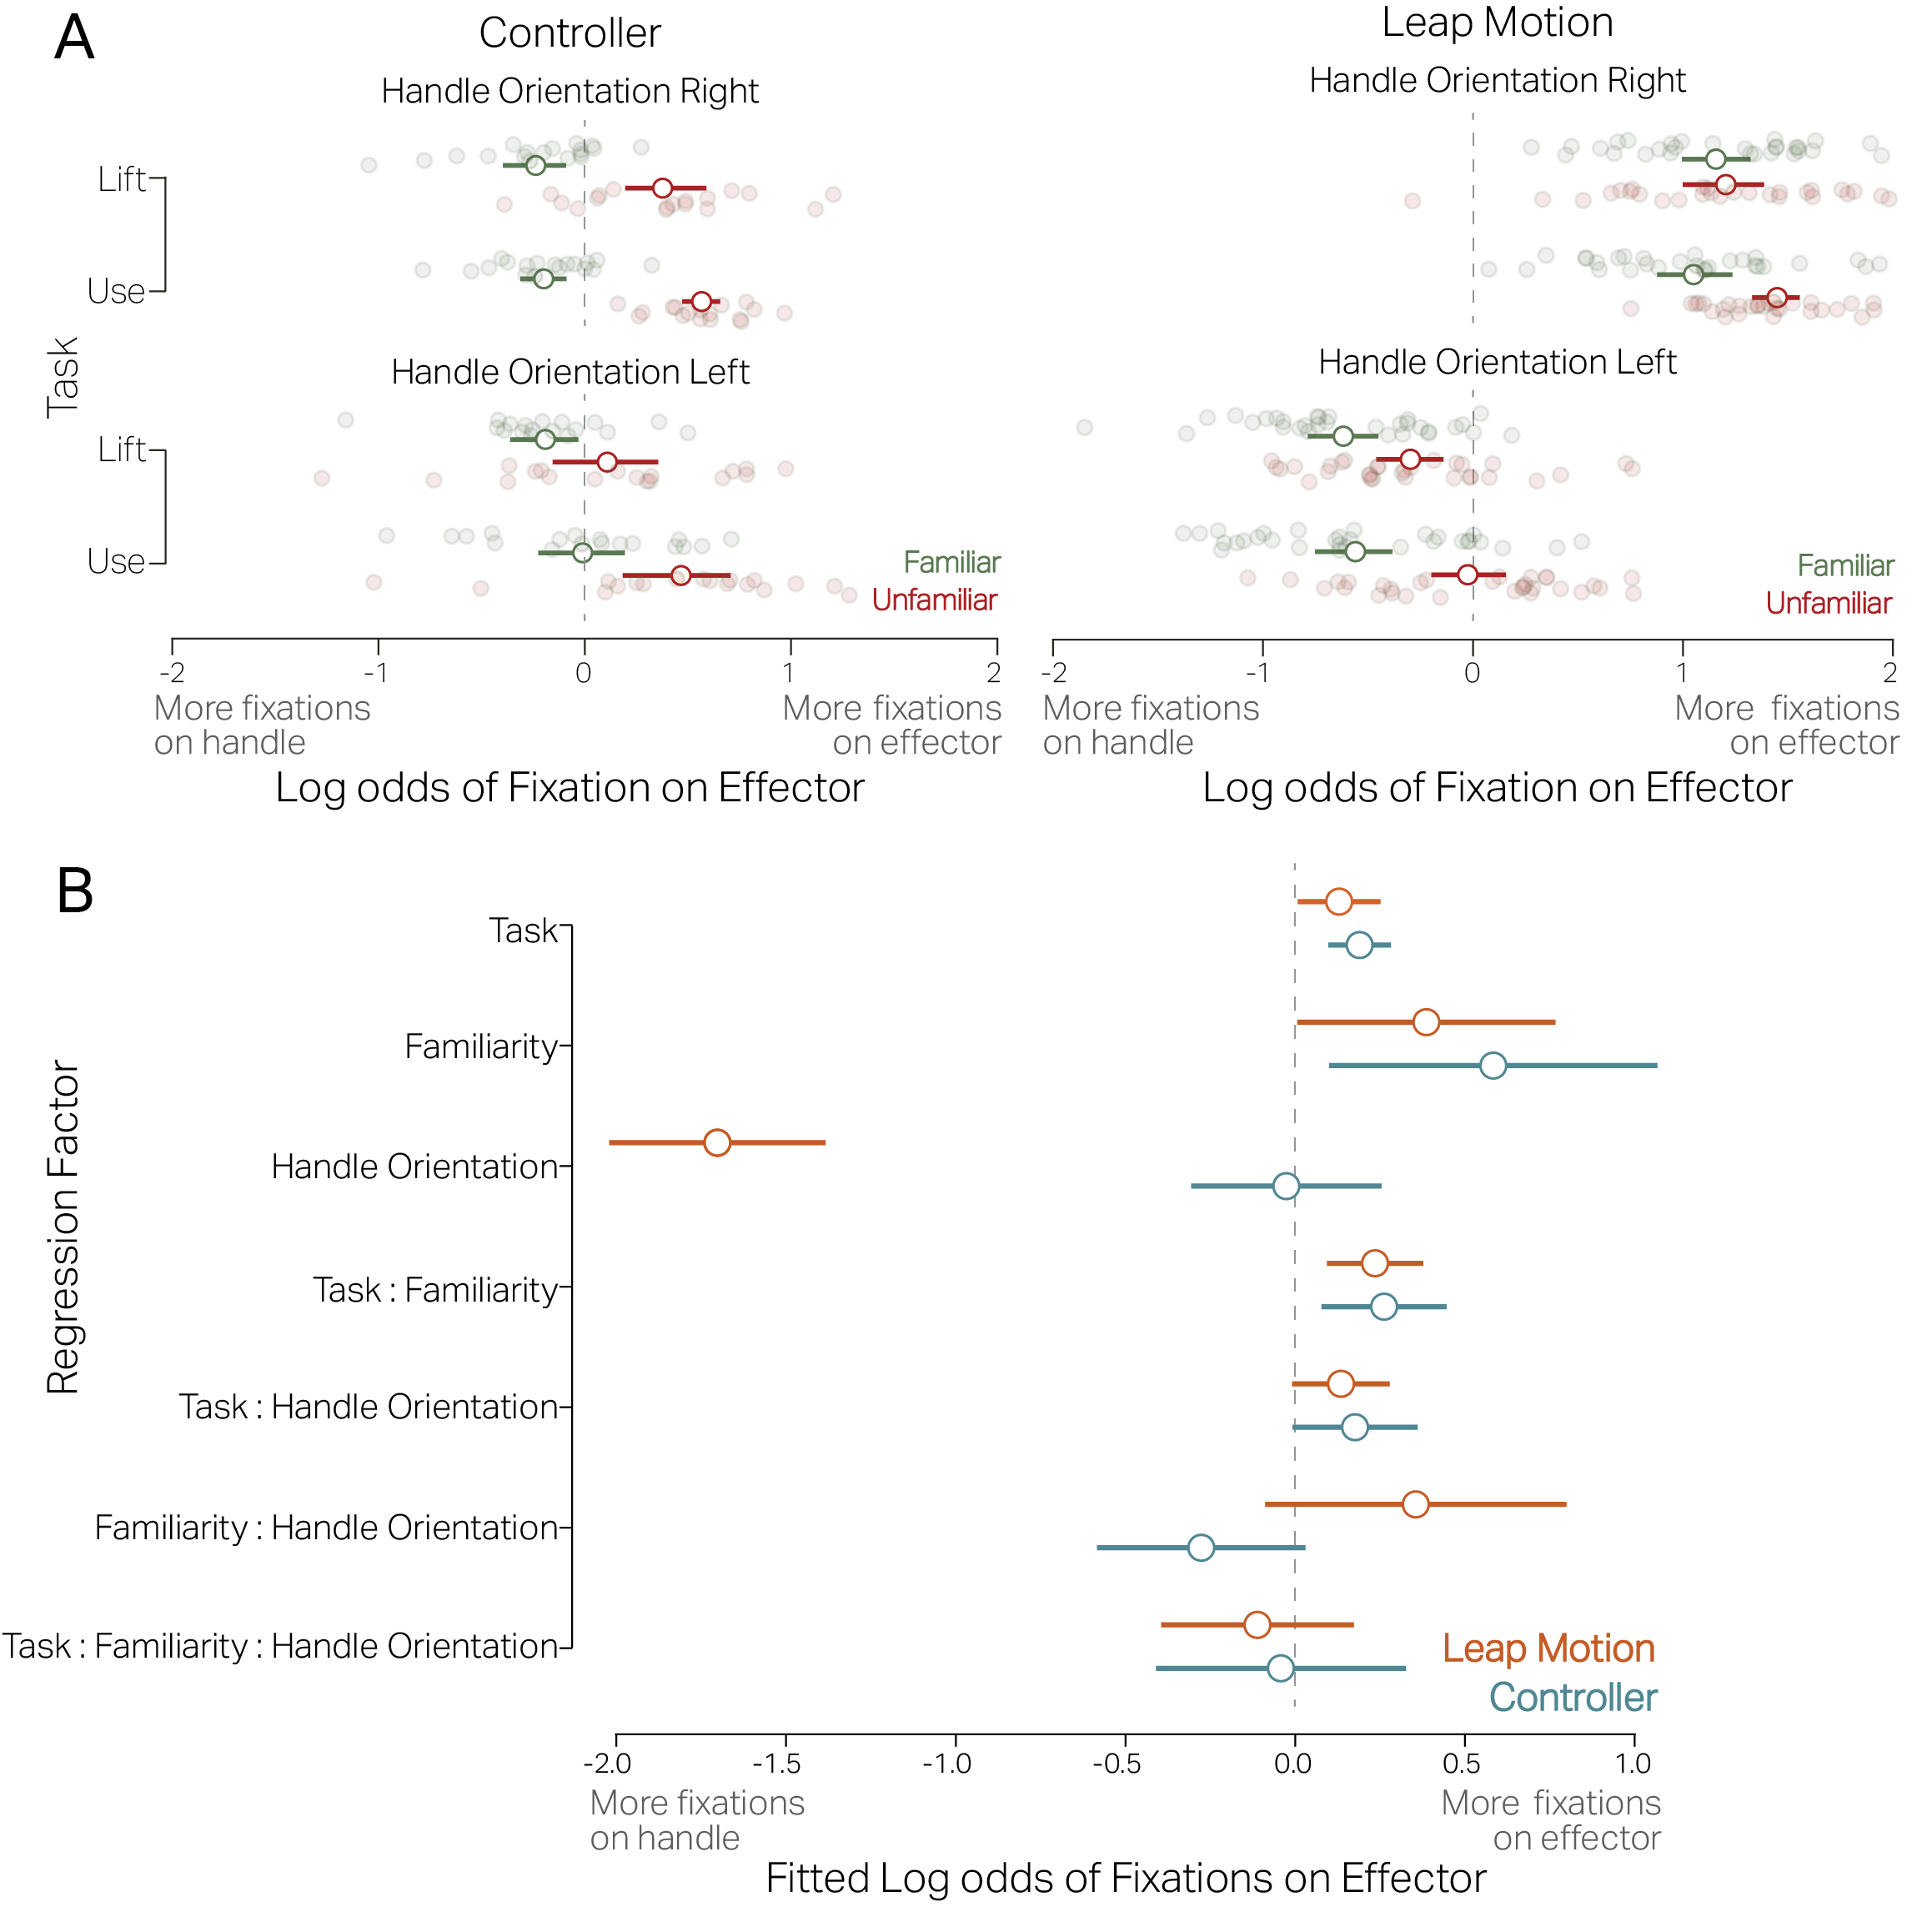
\includegraphics[width=1\linewidth]{source/figures/result/results_combined_logodds.png} \\
    \caption[]{}
    \label{figure:log_odds}
\end{figure}

% \begin{figure}[H]
%     \centering
%     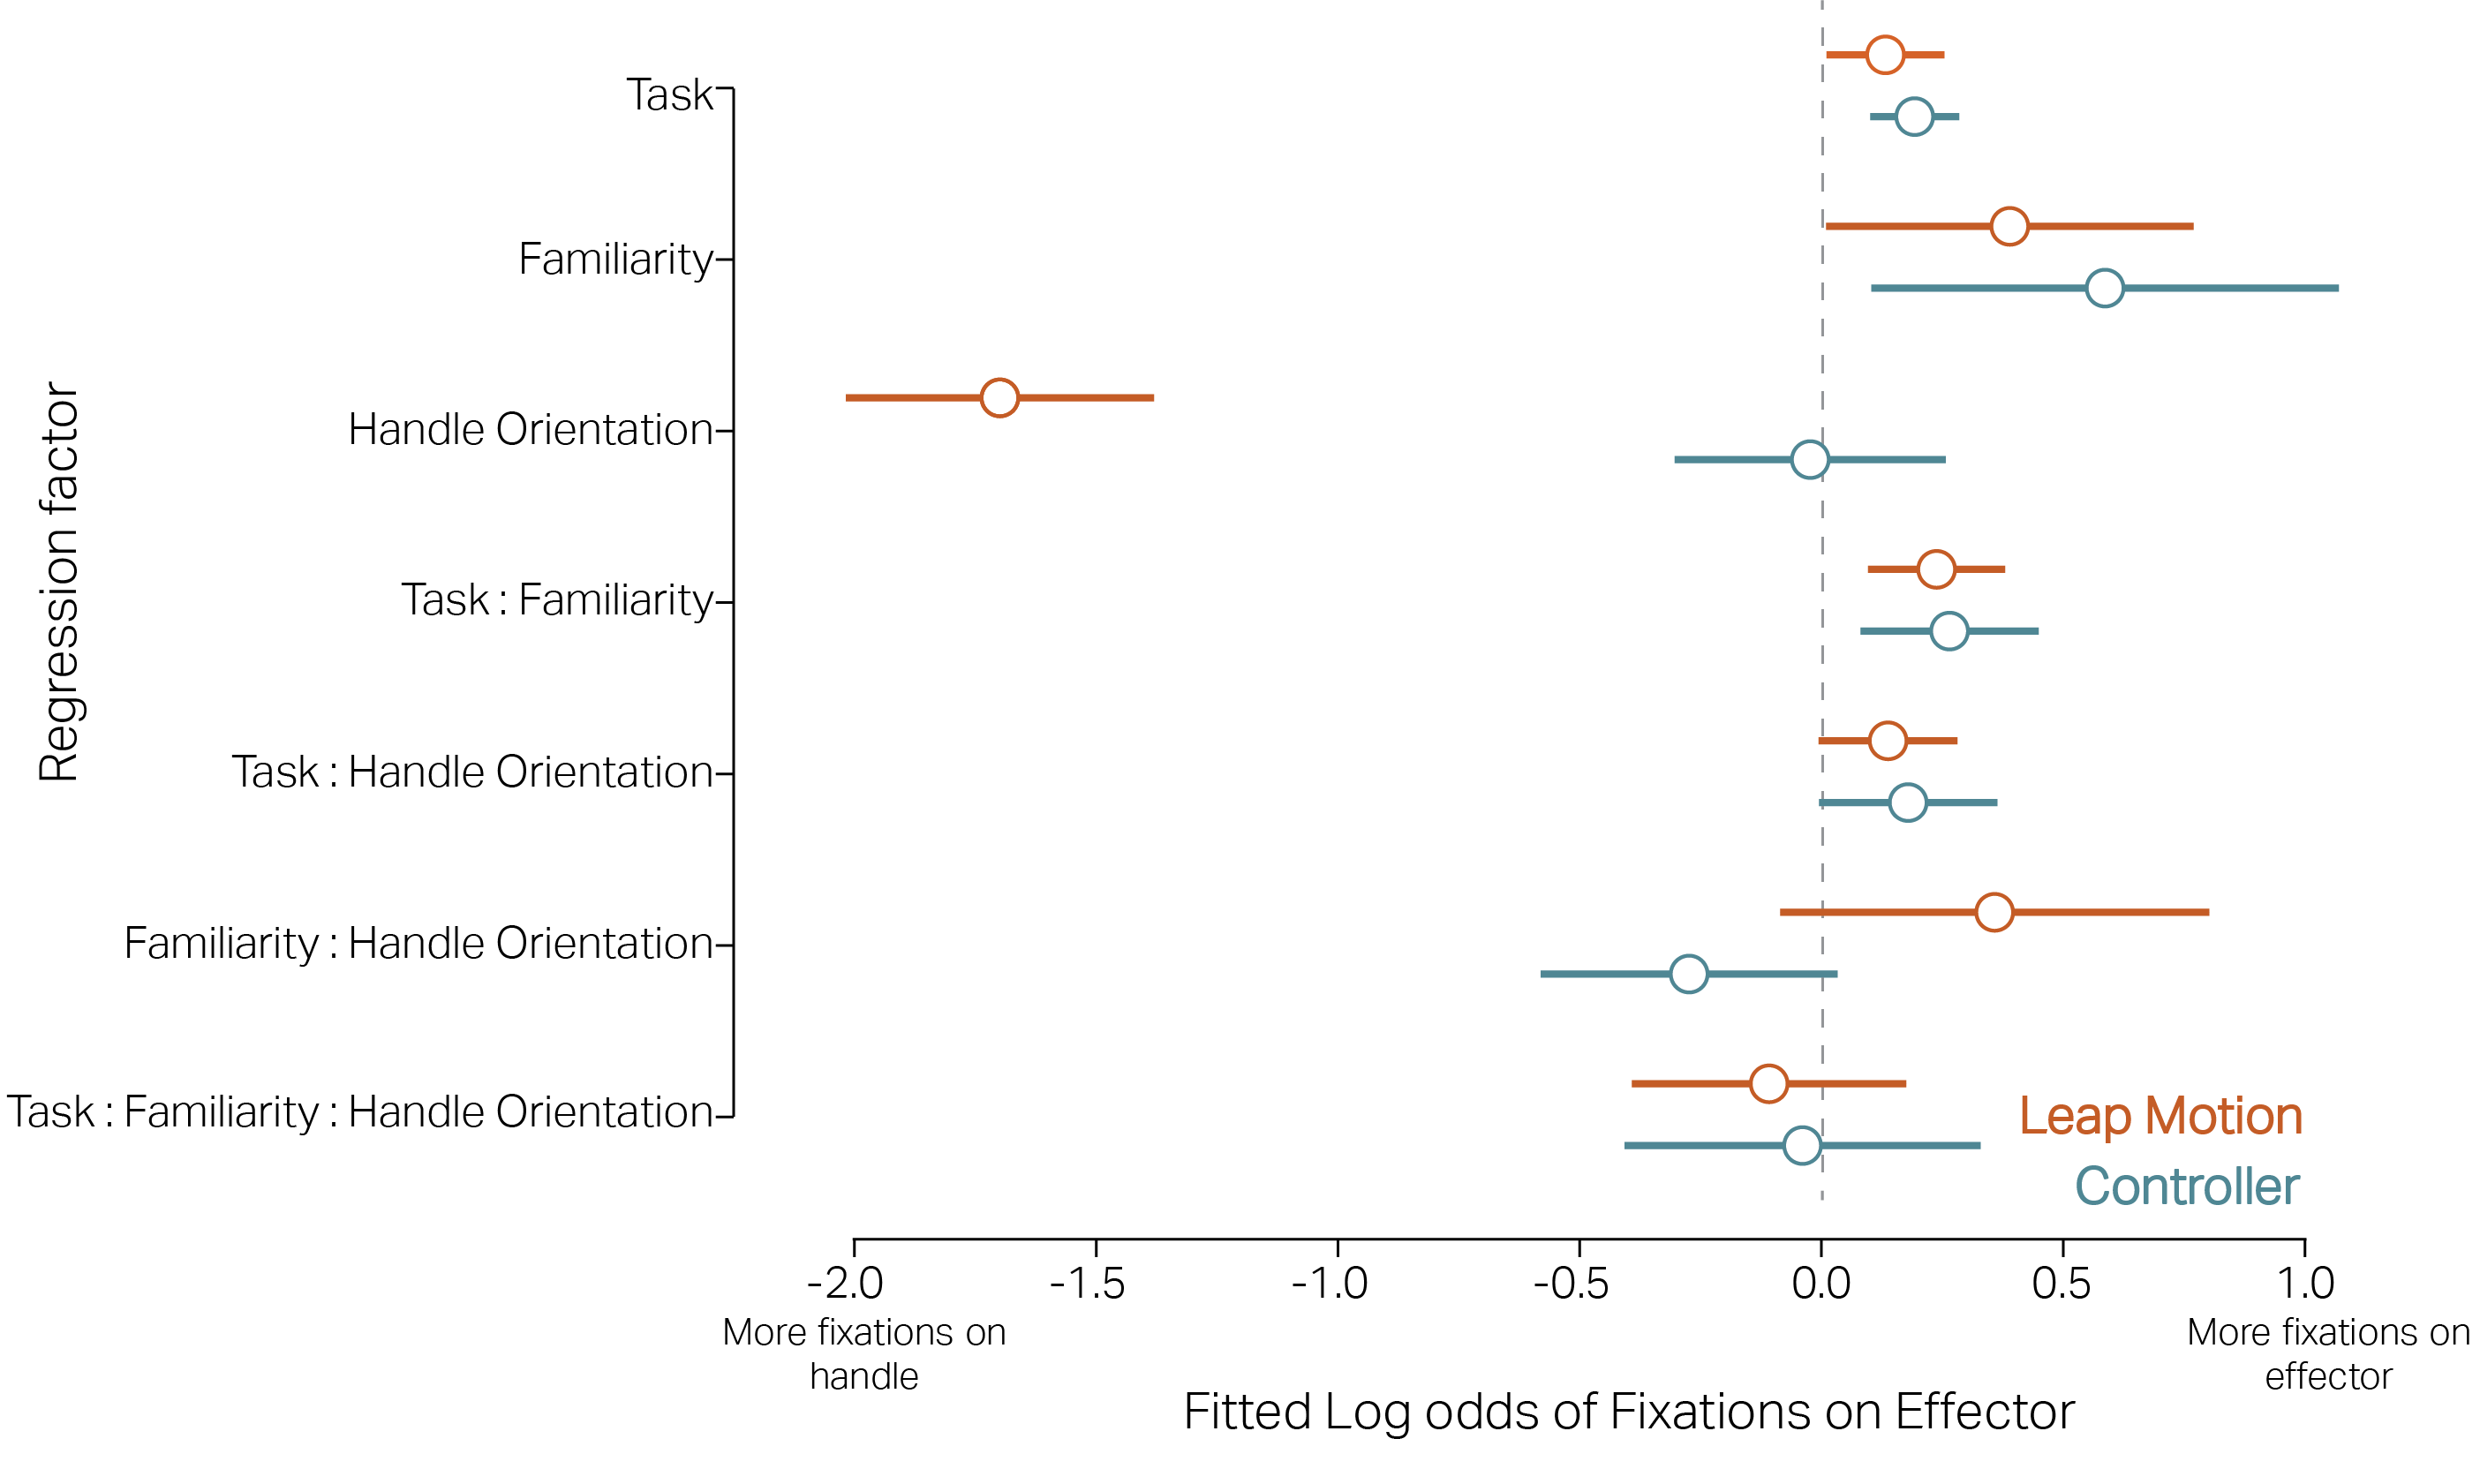
\includegraphics[width=0.7\linewidth]{source/figures/result/model_coefs.png} \\
%     \caption[]{}
%     \label{figure:model_coefs}
% \end{figure}

\begin{figure}[H]
    \centering
    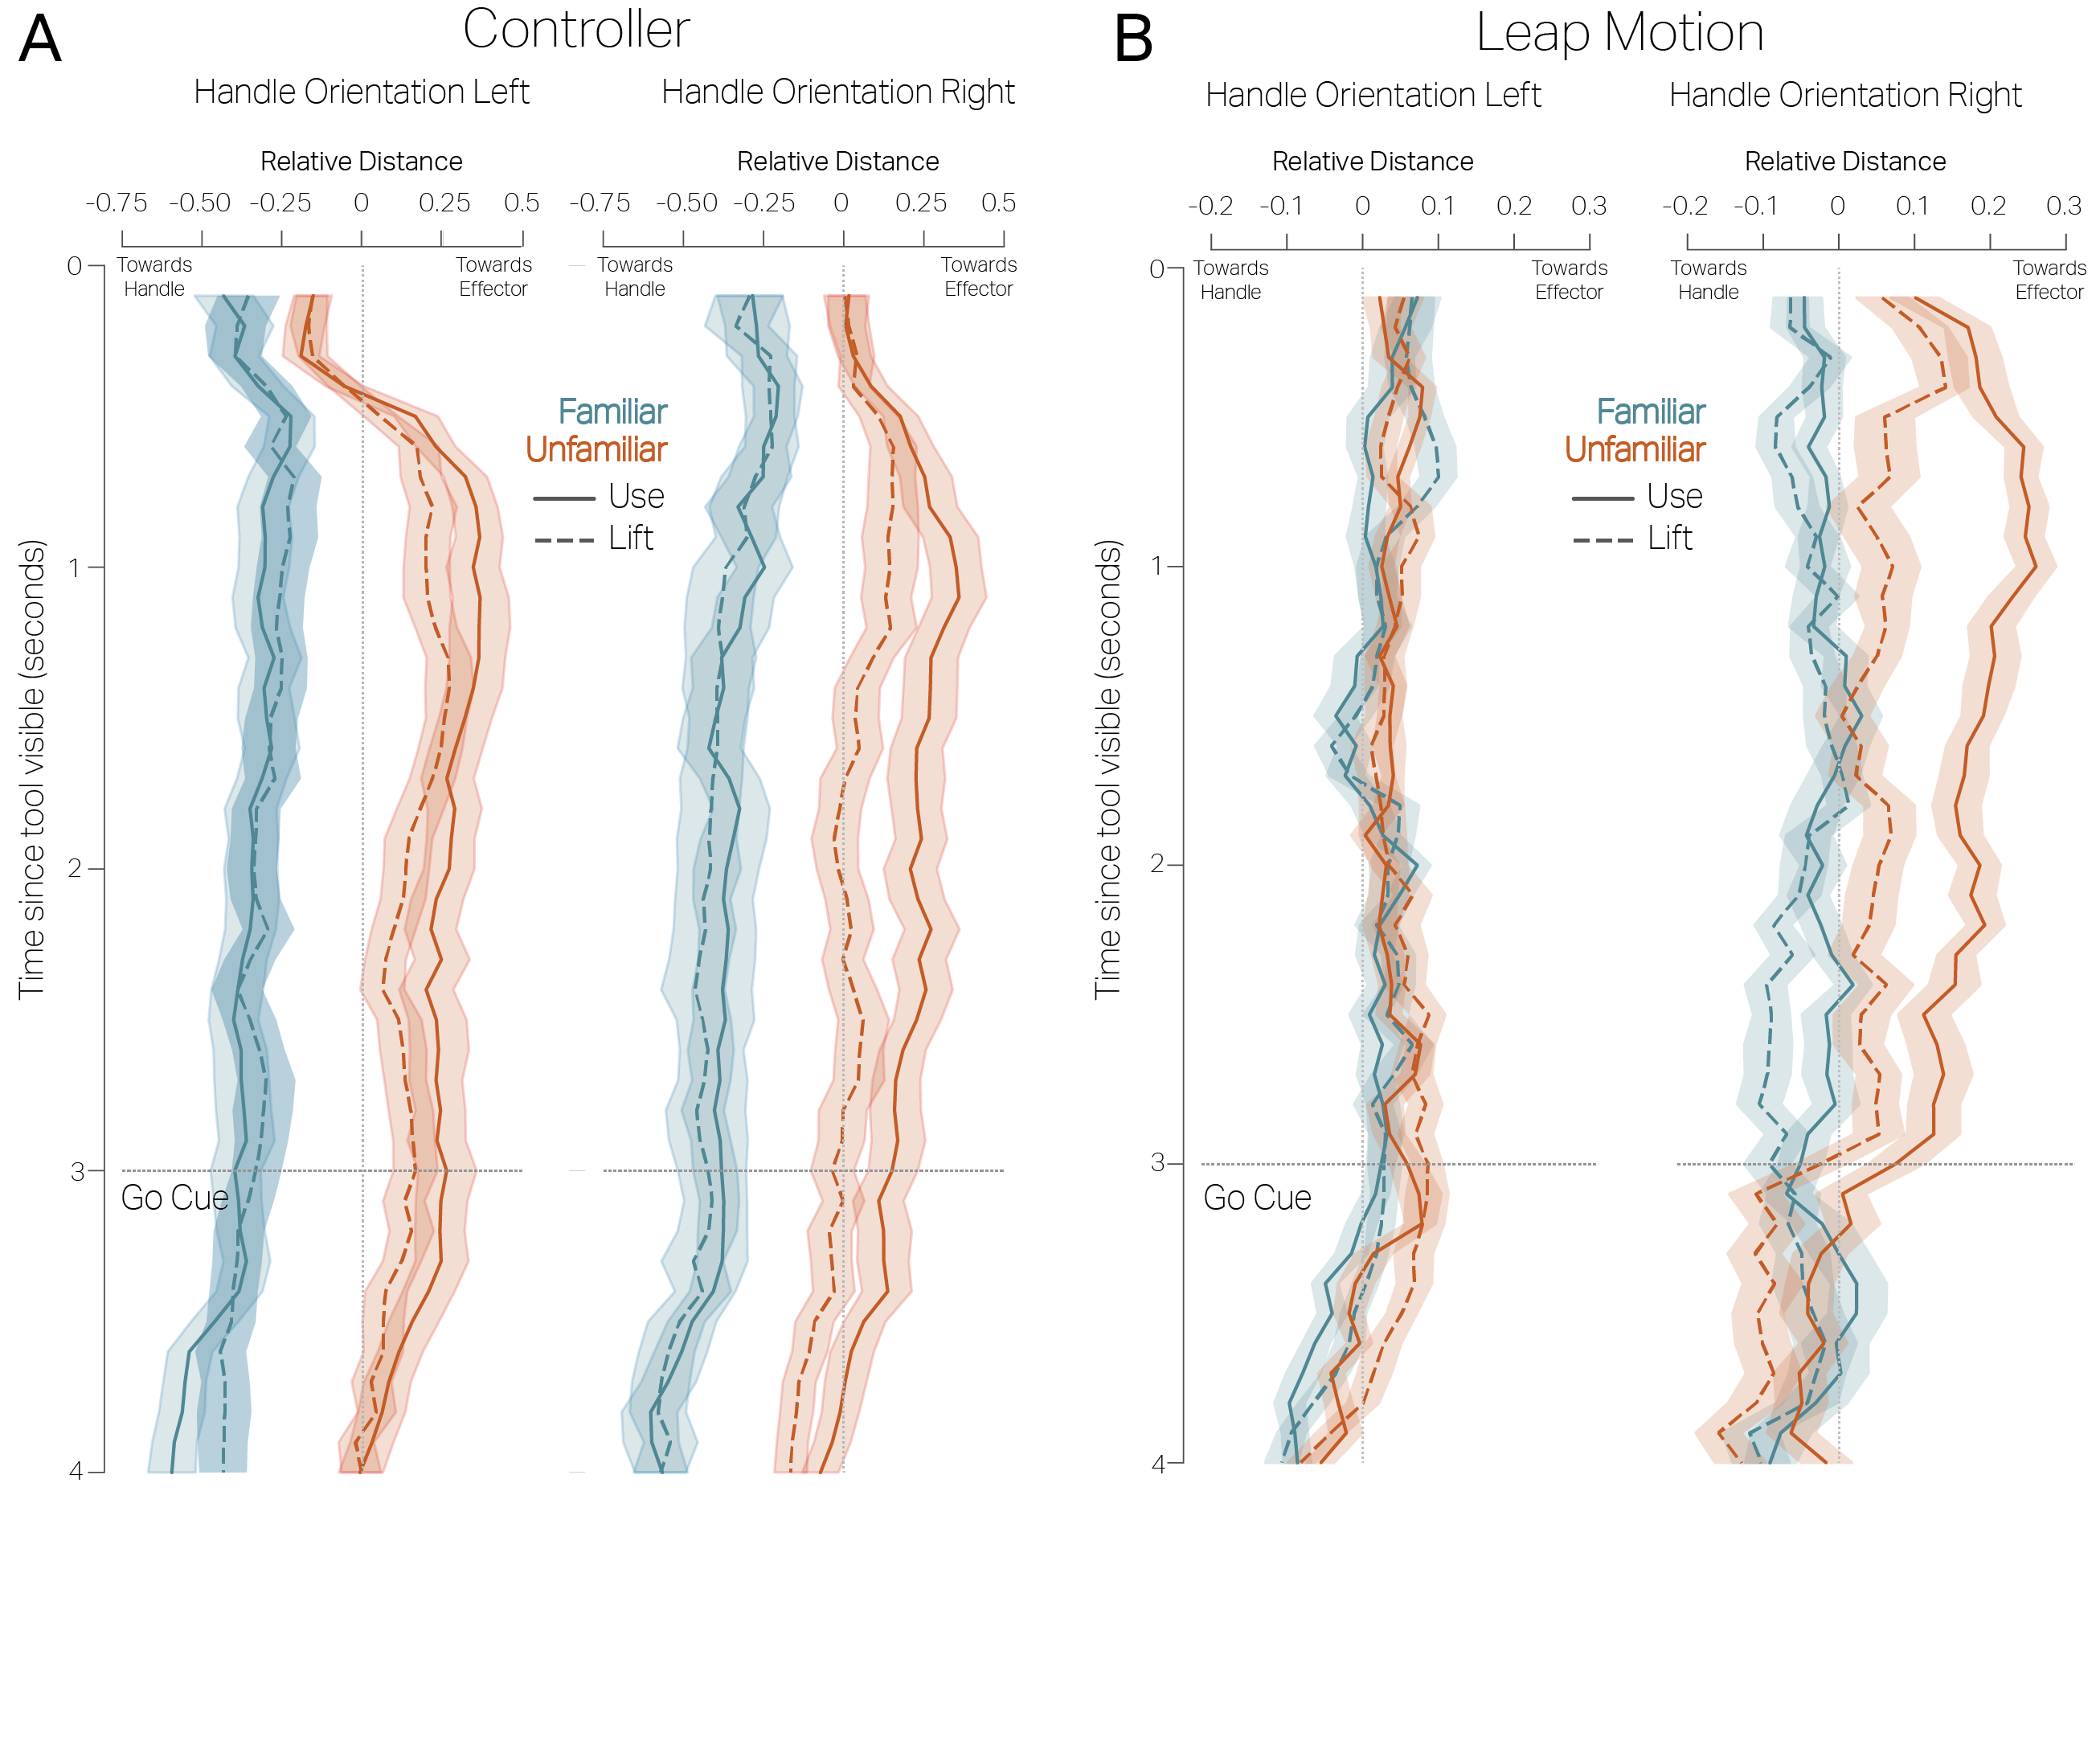
\includegraphics[width=0.7\linewidth]{source/figures/result/deviation_from_center.png} \\
    \caption[]{}
    \label{figure:dev_from_center}
\end{figure}

\begin{figure}[H]
    \centering
    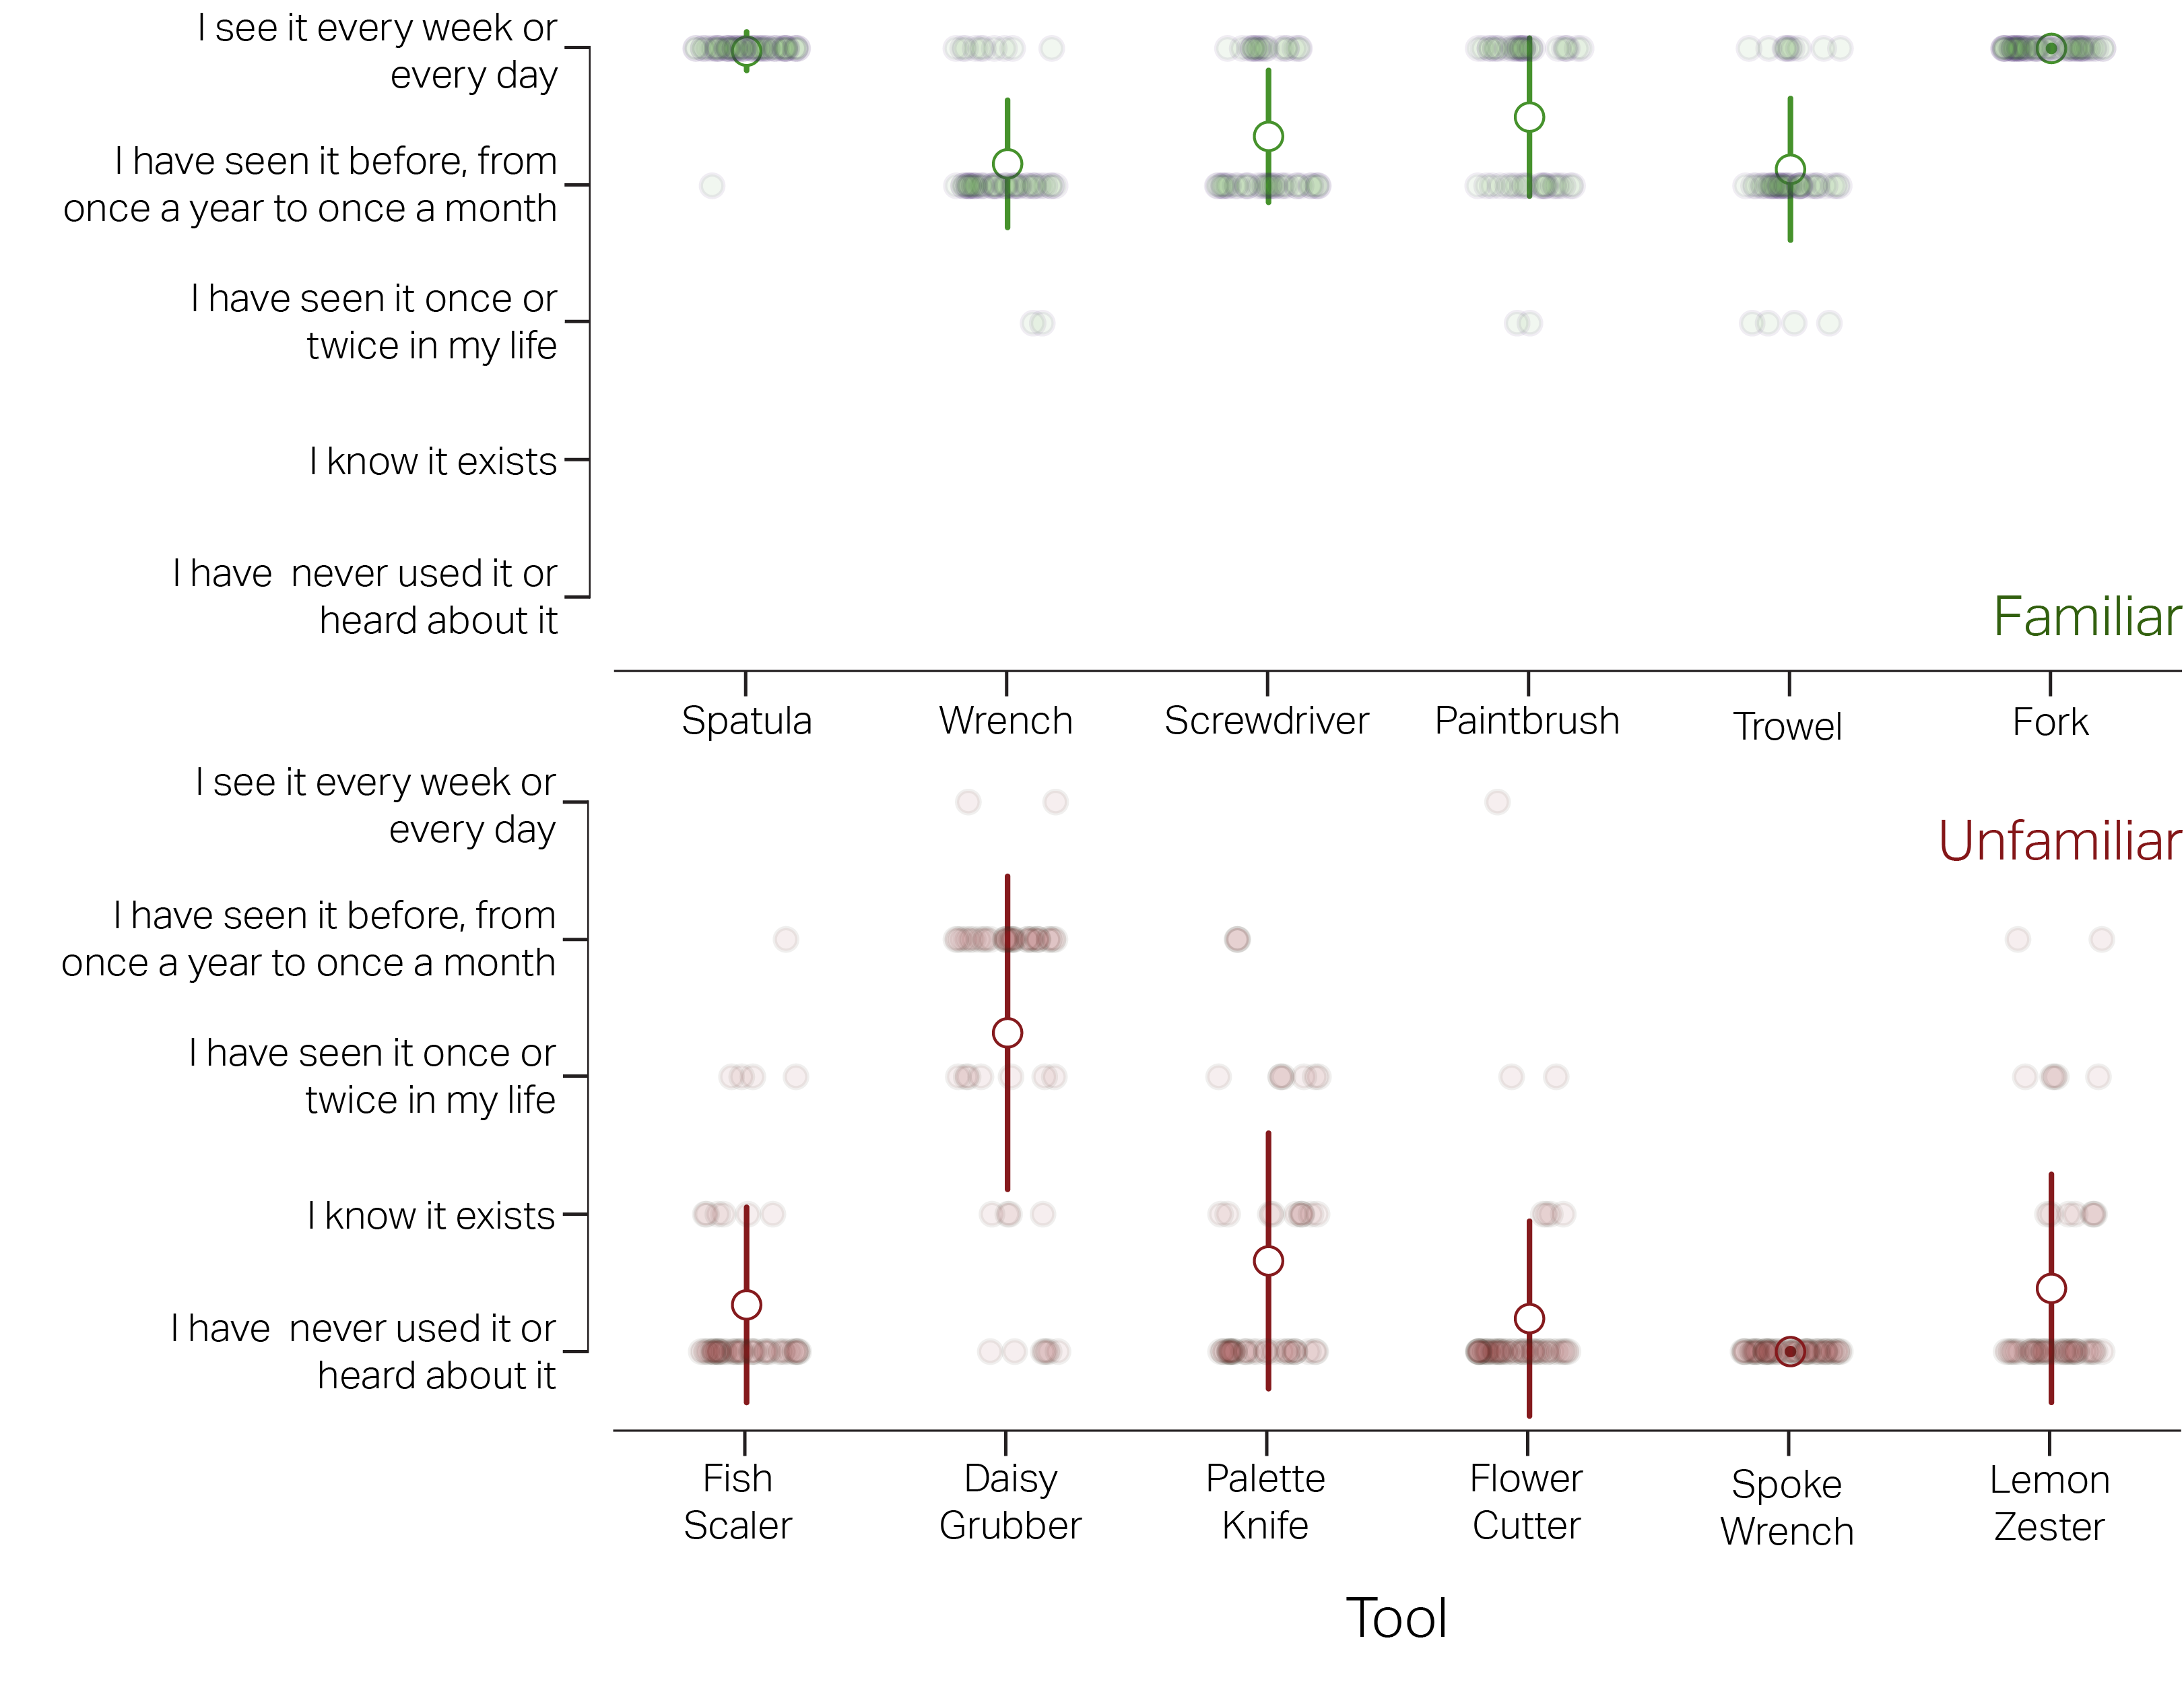
\includegraphics[width=0.7\linewidth]{source/figures/result/familiarity_rating.png} \\
    \caption[]{Participants ratings of their familiarity with the tools used in the study.}
    \label{figure:familiarity_rating}
\end{figure}
\section{Discussion}

The primary aim of this study is to investigate how gaze-based strategies vary for a given task, tool familiarity, and tool handle orientation in naturalistic settings and how the action affordance of the environment can affect this gaze behavior. The factors of the task required the production of tool-specific movements in the case of the use task and generic movements in the case of the lift task. We manipulated the factor of tool familiarity, by presenting tools which were either familiar or unfamiliar. We further controlled the tool orientation with the handle oriented to the right or to the left and were congruent and incongruent to the participants' handedness, respectively. Our experiment design differentiated gaze-based planning and the influence of proximal planning related to grasping the tools and the distal goal-oriented planning of acting with the tools. With our study, we successfully added to the current body of research in two important ways. Firstly, irrespective of the action affordance provided by the interaction methods in the virtual environment, the number of fixations and their eccentricity were modulated by distal goal-oriented factors of task and tool familiarity. When cued to use the tools, there were higher odds of fixating on the effector of the tool as compared to lifting the tool. Similarly, when presented with unfamiliar tools, there were higher odds of fixations on the tool effector as compared to familiar tools. This effect was more pronounced when participants were instructed to use an unfamiliar tool. Secondly, only in the case of naturalistic action affordance that allowed for finer hand and finger movements, anticipatory fixations were significantly biased toward the tool handle when it was oriented incongruent to the subjects' handedness. In sum, our study shows that the action affordance of the virtual environment affects the anticipatory fixations related to proximal goal-oriented planning but not distal goal-oriented planning.

As studies of action-oriented behavior in virtual reality get more popular, there is a need to understand how the interaction methods in the virtual environment can affect behavioral outcomes. In our study, we conducted two experiments to disentangle the role of action affordance for goal-oriented planning. While in experiment-I, participants interacted with 3D tool models using VR controllers which produced a virtual grasp by pulling their index fingers, in experiment-II, participants interacted with tool models by producing an actual grasp. Our results show that the action affordance provided in experiment-II greatly biased the fixations towards the tool handle both in number of fixations and the eccentricity of the fixations when the tool handles were incongruent to the subjects' handedness. These results can be interpreted as fixations being biased to plan grasping the tools when the interaction method affords naturalistic movements. This effect is indicative of an end-state comfort planning \citep{Rosenbaum1996-dq, Herbort2012-ma} where preference is given to the final hand posture rather than a comfortable initial posture. While using VR controllers, such planning is not required as the hand posture is largely fixed. In line with \citet{Pezzulo_undated-gx}, our study shows that anticipatory eye movements can reveal motor planning that selects appropriate movements to achieve the current goal.  

Furthermore, the different interaction methods did not affect distal goal-oriented planning. In both experiments, the odds of sampling visual information from the mechanical properties of a tool are different based on the specificity of the task. Moreover, given tool familiarity, the odds of fixating on the tool effector increased for unfamiliar tools. This effect was more pronounced when subjects were instructed to produce tool-specific movements for unfamiliar tools. These results pertaining to distal goal-oriented planning are in line with the findings reported by \citet{Belardinelli2016-xb}. In our study, we show that well before action initiation, subjects attended to the relevant tool parts to produce the tool-specific actions irrespective of the hand posture afforded by the interaction method.

VR has been poised as a viable method to probe cognitive processing in ecologically valid settings without sacrificing experimental control \citep{Parsons2015-eo}. In our study, we probe how the action affordance of the interaction methods in VR affect planning behavior. Our findings give a fuller view of planning strategies that are needed to produce relevant action. Our study shows that irrespective of the interaction method, semantic and sensorimotor knowledge are inferred from the mechanical properties of the tools as revealed by anticipatory fixations. However, naturalistic actions afforded by the interaction method can bias the anticipatory fixations towards the proximal goals of grasping the tool. Specifically, multiple factors such as semantic and sensorimotor knowledge coupled with end-state comfort planning contribute to anticipatory goal planning. Notably, our study shows that different constraints on the interaction method can also result in different anticipatory behavioral responses. From the perspective of \citet{Gibson1977-zj}, the affordances of the environment are tightly linked to the actions that one can perform in it. Similarly, \citet{ORegan2001-pd} posited that actions constitute the cognitive processes that govern relevant sensorimotor contingencies. Hence, our study offers a veridical and ecological valid context to aspects of anticipatory behavior control.

Studies in eye-hand coordination \citep{Johansson2001-sa, Lohmann2019-fy, Belardinelli2018-xm} have shown that eye movements are proactively made towards the grasp contact points. Furthermore, \citet{Flanagan2006-ql} proposed that predictions are made in an event-oriented manner and are at the heart of successful control strategies for object manipulations. They posit that predicted sensory events are compared with actual events like grasping, lifting, moving the object to monitor task progression. With our study, we make the case that gaze-based predictions are made for action outcomes at different scales, and that eye movements are used to plan both proximal goal of grasping the tools and the distal task-specific requirements well before action initiation. 

Our study adds to the growing body of evidence that anticipation and prediction are at the core of cognition \citep{Pezzulo2007-ot}. Motor theories of cognition have proposed that simulations of actions reuse internal models of motor commands to effect multiple predictions \citep{Jeannerod2006-dt}. The simulation of action theory has been used to explain numerous phenomena of planning, prediction of external events, visual perception, and imitation. \citet{Hoffmann2003-ur} introduced anticipatory behavior control as the mechanism by which action-effect representations are activated by the need for an effect-related goal and contingent stimuli. Furthermore, \citet{Pezzulo2021-te} recently proposed that generative models provide top-down predictive signals for perception, cognition, and action during active tasks and these signals are otherwise weak and/or absent when the brain is at rest or the stimuli are weak. Our study shows that anticipatory behavior is tightly linked to the production of task-relevant actions and is contextualized to the action affordance of the environment.

We conducted the present study in virtual reality, which is still a burgeoning technology for vision research. While VR environments pose an exciting avenue of research, there are still limitations that practitioners must face while conducting experiments. First, the naturalistic setting of both experiments I and II afforded natural head movements. To maintain optimal quality over the data, we asked the participants in the study to make limited head movements. Additionally, we presented the tools and the task cues not to cause extreme pitch head movements. Secondly, mobile eye-trackers can be error-prone and might suffer from variable sampling rates \citep{Ehinger2019-xr} or calibration errors due to slippage \citep{Niehorster2020-yq}. To mitigate any calibration errors, we also made sure that we calibrated the eye-trackers at regular intervals. Thirdly, both controller-based and camera-based VR interaction methods are still new technology. It could have been challenging for participants to get used to, even though we made sure they practiced the interaction before the experiment. While we simulated grasping the tool using LeapMotion’s gesture recognition and were able to produce a more realistic actions, it is still an inadequate substitute for a real grasp where the tactile feedback of the tool in hand might elicit more accurate responses. For example,\citet{Ozana2018-ih} showed that grasping movements within a virtual environment differ both quantitatively and qualitatively from typical grasping. Lastly, while there are visible differences between the environments, we see that there are no significant differences between the percentage of fixations allocated to the tool and the rest of the environment in both the experimental settings. Hence, we contend that the differences in the eye movement behavior reported in the study are largely a consequence of the differences in the action affordance and much less because of mere visual differences of the environments. In light of these limitations, we know that our study must be considered from a nuanced perspective. Furthermore, there is still room for replicating our study with novel and more realistic interaction methods.

There are still some open questions pertaining to anticipatory behavior elicited by tool interactions. Firstly, while our study distinguishes between levels of action affordances, future work can look at goal-oriented planning for passive observers at both proximal and distal levels. Secondly, it would be interesting to dive deeper into the predictive neural signals that give rise to the present oculomotor behaviors. Our study provides a first step towards distinctly investigating proximal and distal goal-oriented planning.

\section{Conclusion}

The present study gives a veridical and ecologically valid context to planning and anticipatory gaze behavior. Our results support the hypothesis that eye movements serve the cognitive function of actively sampling information from the environment to produce relevant actions. When semantic information about the object is not readily available, eye movements are used to seek information from its mechanical properties from specific locations. Furthermore, we show that fixations are made in a goal-oriented way in anticipation of the relevant action. When considering the realism of the action affordance, our results show that eye movements are affected by both proximal goals of manually grasping objects and the distal task-based demands. Lastly, our study is at the frontiers of naturalistic vision research, where novel technologies can be harnessed to answer questions that were previously far-fetched.



\section*{Acknowledgement}
We are grateful for the financial support by the German Federal Ministry of Education and Research for the project ErgoVR (Entwicklung eines Ergonomie-Analyse-Tools in der virtuellen Realität zur Planung von Arbeitsplätzen in der industriellen Fertigung)-16SV8052. 

\bibliographystyle{plainnat}
\bibliography{ErgoVR_references}
% \appendix

% \section{APPENDIX}

\begin{figure}[h]
    \centering
    \subfloat[]{\includegraphics[width=0.5\linewidth]{source/figures/results/fixations_between_grasps.png}
    \label{figure:fix_bw_grasp}} 
    \subfloat[]{\includegraphics[width=0.4\linewidth]{source/figures/results/lookahead_distance_most_fixated.png}
    \label{figure:most_fixated}}\\
    \subfloat[]{\includegraphics[width=0.4\linewidth]{source/figures/results/lookahead_distance_duration_easy.png}
    \label{figure:tla_easy}}
    \subfloat[]{\includegraphics[width=0.4\linewidth]{source/figures/results/lookahead_distance_duration_hard.png}
    \label{figure:tla_hard}}
    \caption[]{\protect\subref{figure:fix_bw_grasp} shows the probability density of unique objects fixated on between consecutive grasps for the two trial types EASY (blue) and HARD (red). For both EASY and HARD trials, maximum probability density of fixation is on three unique objects in the scene. \protect\subref{figure:most_fixated} shows the probability density of the most fixated object in a grasp sequence. For both EASY and HARD trials, the maximum probability of density is on the object that is immediately grasped next, this shows that between two grasp onsets, maximum attention is allotted to the object that is next in line to be grasped. 
    \protect\subref{figure:tla_easy}\protect\subref{figure:tla_hard} show the joint probability density of the dwelling time (total fixation duration) on an object between consecutive grasps and it's position in the relative grasp sequence for EASY and HARD trials respectively. The figure also shows the marginal probability density of the dwelling time  on an object and it's relative position in grasp sequence. The abscissa refers to the relative grasp sequence of a fixated object i.e., when the grasp sequence of a fixated object is 1 the object is grasped next or when the grasp sequence is 2 the fixated object is grasped one after the next grasp.  the The figure shows that the dwelling time is highest on the object that is immediately next in line to be grasped. The dwelling time reduces linearly on the objects that are upcoming in the relative grasp sequence. The differences in the EASY and HARD trials can be explained by the higher number of objects fixated on between grasps in the HARD trials as shown in \protect\subref{figure:fix_bw_grasp}
    }
    \label{figure:planning_behavior}
\end{figure}


\begin{figure}[h]
    \centering
    \subfloat[]{\includegraphics[width=0.3\linewidth]{source/figures/results/t50_easy_execution.png}
    \label{figure:t50_easy_exe}}
    \subfloat[]{\includegraphics[width=0.3\linewidth]{source/figures/results/t50_hard_execution.png}
    \label{figure:t50_hard_exe}} \\
    \caption[]{Cumulative distributions of time of first fixation on the 7 regions of interest for the action execution epochs. The dotted line indicates time required in 50\% of all epochs to first fixation on the ROIs. The time taken for first fixation on each ROI can be  used to determine the attention attraction power of a region of interest i.e. the time taken to saccade to the region of interest.\\
    Panel \protect\subref{figure:t50_easy_exe} shows the cumulative plots for the 7 ROIs for the EASY trials. In 50\% of the action execution epochs the 7 ROIs are fixated on within half time of the epoch duration. At the 50\% mark, the curves indicate the latency of gaze shift from the current\_TO, other objects and shelves, closely followed by the previous target object and shelf (prev\_TO, prev\_TS), then to next target shelf (next\_TO), current target shelf (current\_TS) and next target object (next\_TO). This is indicative of attention equally distributed on the 6 ROIs and no selective preference for any one object or shelf in the task sequence during the later stages of action execution epoch.\\
    Panel \protect\subref{figure:t50_hard_exe} shows the cumulative distribution of the time to first fixation on the 7 ROIs for HARD trials. In 50\% of the action execution epochs, a similar trend is seen as in the EASY trials.
    }
     \label{figure:t50_overall_exe}
\end{figure}



\begin{figure}[h]
    \centering
    \subfloat[]{\includegraphics[width=0.25\linewidth]{source/figures/results/t50_easy_planning.png}
    \label{figure:t50_easy_plan}}
    \subfloat[]{\includegraphics[width=0.25\linewidth]{source/figures/results/t50_hard_planning.png}\label{figure:t50_hard_plan}}
    \caption[]{Cumulative distributions of time of first fixation on the 7 regions of interest for action planning epoch. The dotted line indicates time required in 50\% of epochs to first fixate the ROIs.
    Panel \protect\subref{figure:t50_easy_plan} shows the cumulative plots for the 7 ROIs for the EASY trials. In 50\% of the epochs gaze is directed early to the previous target object and shelf. Further, gaze moves to other objects/shelves in the scene which is then followed by close fixations on next target object and shelf and lastly to the current target object well before the action on the object is executed. This is indicative of attention sequentially moving from one ROI to the next.
    Panel \protect\subref{figure:t50_hard_plan} shows the cumulative distribution of the time to first fixation on the 7 ROIs for HARD trials. In 50\% of the grasp epochs, The latency of first fixations on the ROIs remains roughly similar to the action planning epochs of the EASY trials, where the early fixations are on the previous target object and shelf and the last on the current target object before being manipulated.}
     \label{figure:t50_overall_plan}
\end{figure}
\end{document}


